\section{Soya Basics}
This section will guide you through the basics of using Soya. 

\begin{notice}
It is \emph{highly} recommended you get the Soya tutorial package. It contains
alot of information directly from the authors of Soya. 
\end{notice}

\subsection{Setting up a basic scene}
At the end of this section you should be able to load and display a simple model. 
You can also refer to \file{soya_tutorials/basic-1.py}.

To display a simple 3D model we need the following things:
\begin{itemize}
  \item a scene, to group all the objects together
  \item a model
  \item a light
  \item a camera
\end{itemize}

First we will look at the very bare bones of a soya script:
\begin{verbatim}
import os
import sys
import soya

soya.init()

soya.path.append('data')

# ...
\end{verbatim}

\code{soya.init()} is called to initialize soya and its globals. 

\code{soya.path.append('data')} is to tell soya where to search for models,
images, fonts etc. It is often required that the data files are going 
to be relative to the script. To handle such situations something like this is
often used:

\begin{verbatim}
soya.path.append(os.path.join(os.path.dirname(__file__), 'data'))
\end{verbatim}

The next step is to create a scene object. The scene is a \class{soya.World}
which will contain our 3D objects. You can think of a world as a group of 3D
objects. 

\begin{verbatim}
scene = soya.World()
\end{verbatim}

Now we will load our model into a \class{soya.Shape}. The model file needs to
be in \file{data/shapes/your_model.data}. To create the model you need to use 
blender and use the \file{blender2soya.py} script included with soya. 

Once we have our shape we can put it into a \class{soya.Volume}. 
The first argument to \class{soya.Volume}'s constructor is its parent. This 
must be a \class{soya.World} object or None. The second argument is our shape.

\begin{verbatim}
sword_shape = soya.Shape.get("sword")
sword = soya.Volume(scene, sword_shape)
\end{verbatim}

The sword object can now be moved and rotated freely ( all relative to its
parent ). For example to move our object around a bit we could do:

\begin{verbatim}
sword.x = 1.0
sword.y = -0.4
sword.z = 1.0
\end{verbatim}

Of course if you need to set x, y and z all at the same time you can use 
the helper function \function{volume.set_xyz(1.0, -0.4, 1.0)}.

So our model is loaded and ready, next we need light. Creating a light 
is very similar to creating any object in soya. 

\begin{verbatim}
light = soya.Light(scene)
light.set_xyz(0.4, 0.0, 2.0)
\end{verbatim}

If you have understood everything so far creating a camera is no problem:
\begin{verbatim}
camera = soya.Camera(scene)
camera.z = 2.0
\end{verbatim}

The camera object is slightly more complex however. We must tell soya that 
we want to use camera as the \emph{root widget}. It is possible to use 
other things as root widget's for overlayed 2d displays and split screen etc. 
But for now you just need to know that you need to do:
\begin{verbatim}
soya.set_root_widget(camera)
\end{verbatim}

All our objects are now created. The only thing left to do is create an 
instance of \class{soya.Idler}. A \class{soya.Idler} manages your scene objects
and is basically the 'main loop' for your application. It will also, by default, 
regulate the frame rate to 40 FPS. 

\begin{verbatim}
soya.Idler(scene).idle()
\end{verbatim}

\subsection{Basic Animation and Rotation}

You may want to look at \file{soya_tutorials/basic-2.py} for this section. 

All objects descended from \class{soya.CoordSyst} (which is just about 
everything) have rotation and location functions/attributes. The 
previous section demonstrated some of the location methods, this section
will demonstrate the rotation methods and how to use them to produce 
simple animation. 

The basic rotation functions are:
\begin{itemize}
  \item \function{rotate_lateral}: rotate around the Y axis
  \item \function{rotate_vertical}: rotate around the X axis
  \item \function{rotate_incline}: rotate around the Z axis
\end{itemize}

\begin{notice}
Think it sounds very confusing? Why not just just rotate_x, rotate_y, 
rotate_y? Good question ;)
\end{notice}

We will now extend \class{soya.Volume} to make \class{RotatingVolume}.
We will use the \function{advance_time} method. There are 3 time related
functions you can use for all Soya objects:
\begin{itemize}
  \item \function{begin_round}
  \item \function{end_round}
  \item \function{advance_time}
\end{itemize}

One \emph{round} is 30 milliseconds ( by default ). \function{advance_time}
is called 1+ times per round with a proportion argument. If for 
example the proportion is 0.3 then 30\% of the round has occured. (ie.
0.9ms). Therefore is preferential to do animation in the advance_time 
method. 

\begin{verbatim}
class RotatingVolume(soya.Volume):
  def advance_time(self, proportion):
    # call the super implementation.
    soya.Volume.advance_time(self, proportion)

    # rotate around the Y axis with an amount proportional to proportion
    self.rotate_lateral(proportion * 5.0)
\end{verbatim}

\subsection{Creating models with Blender}
This section will guide you through creating and exporting a simple textured 
model from Blender. 

\begin{notice} 
  It is presumed you are familiar with the basics of using Blender. For an
  introduction to Blender see 
  \url{http://download.blender.org/documentation/htmlI/}
\end{notice}

In this section we will create a simple textured cube. So create a cube:

\includegraphics[scale=0.6]{blendertut/atut1.eps}

Return to \emph{Object Mode} and create a new material. 

\includegraphics[scale=0.6]{blendertut/atut2.eps}

Add to this your texture image. 

\begin{notice}
  For your texture to work with soya its dimensions must be $n^2$ ( ie. 64x64,
  128x128, 512x512, ...)
\end{notice}

You should place the texture into \file{data/images/yourTexture.something}.
You should, but don't have to, keep your blender files in \file{data/blender}. 
Using blender's relative path feature, you can then set the image
file as \file{//../images/yourTexture.something}, enabling other designers
to edit your model without having to re-adjust all the paths. 

\includegraphics[scale=0.6]{blendertut/atut3.eps}

Presuming you want to use UV co-ordinates ( you probably do ) you then need to 
toggle the UV button on the Map Input tab.

\includegraphics[scale=0.6]{blendertut/atut4.eps}

We now split the blender windows so we can view the UV editor and the 3D window.

In the 3D window enter face select mode either using the drop down or by 
pressing the F key. Press A or use the menu to select all faces. 

\includegraphics[scale=0.6]{blendertut/atut6.eps}

Now in the UV image window use the drop down to select the texture image name. 
The texture should appear in the window. 

\includegraphics[scale=0.6]{blendertut/atut7.eps}

You can now leave Face select mode ( again by pressing F or using the dropdown). 
Changing the view type to Textured you should be able to see your textured model. 

\includegraphics[scale=0.6]{blendertut/atut8.eps}

Now is a good time to save your model again. 

Change the window type of the UV window to Text Editor. Use File -> Open to 
load the \file{blender2soya.py} script. Press Alt+P to execute the script 
or use the menu. 

You will be presented with a GUI allowing you to select export options. 
The Path option should be set to your \file{data} directory. 

\includegraphics[scale=0.6]{blendertut/atut9.eps}

Thats it! You may be thinking this seems a lot of work each time you make 
changes to your model... and so did the author of Soya. If you have kept 
your blender models in \file{data/blender} and blender is in your system
path, Soya will automatically call blender and the export script if the 
blender file is newer than the exported model. You can think of this 
as an automatic export. 


\subsection{Soya's Base Classes}

This section will describe some of soya's base classes. 

Here is a small diagram to help you understand the class hierachy for soya:

\begin{figure}
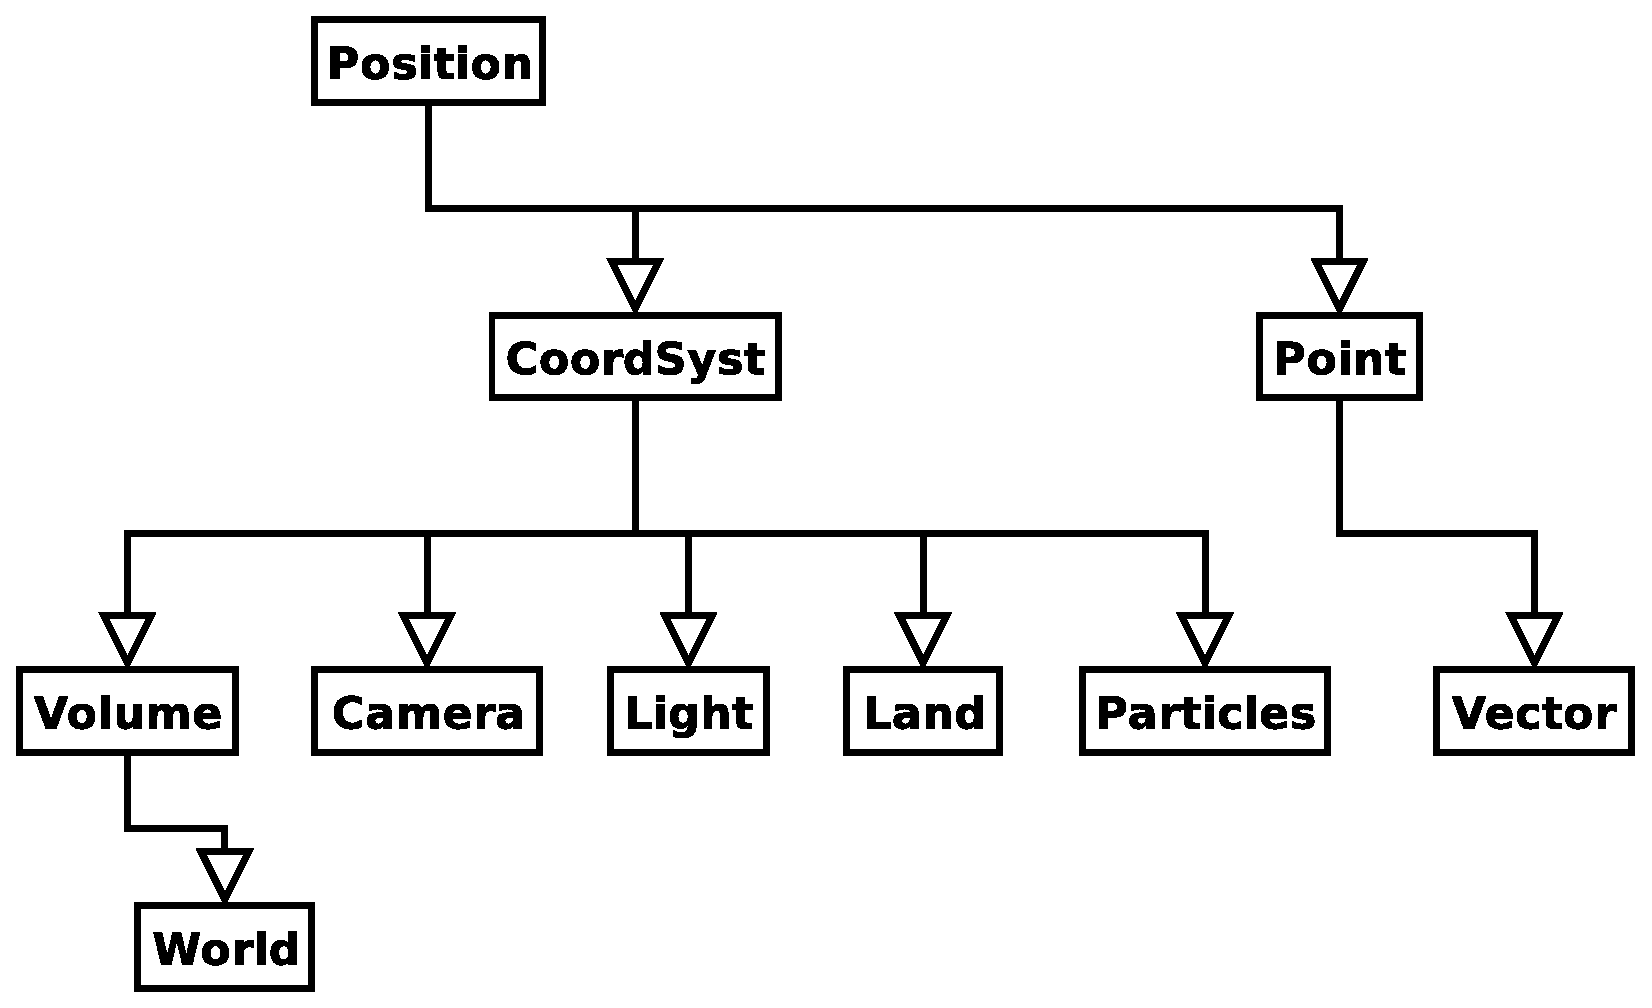
\includegraphics[scale=0.4]{classes.eps}
\end{figure}

\class{soya.Position} is an abstract class so you dont need to worry about it. 

A \class{soya.Point} is just a 3D position. It is used for math computation but
it \emph{doesn't} display anything. 

\class{soya.Point} has x, y and z attributes. It also has a parent attribute. 
If you have read the earlier sections this should sound very familiar. 
For example:

\begin{verbatim}

>>> scene = soya.World()
>>> p = soya.Point(scene)
>>> p.x
0.0
>>> p.y
0.0
>>> p.z
0.0
>>> p.x = 5.0
>>> p.x
5.0
>>> p.set_xyz(1.0, 2.0, 3.0)
>>> p.x, p.y, p.z
(1.0, 2.0, 3.0)
>>> p.parent
<World, shape=None>
>>> p
<Point 1.0, 2.0, 3.0 in <World, shape=None>>

\end{verbatim}

It is also possible to move objects straight to the location of another object
( we use here the other arguments to \class{soya.Point} to specifiy the initial
location ):

\begin{verbatim}
>>> p1 = soya.Point(scene, 0, 10, 0)
>>> p2 = soya.Point(scene, 1, 2, 3)
>>> p1
<Point 0.0, 10.0, 0.0 in <World, shape=None>>
>>> p2
<Point 1.0, 2.0, 3.0 in <World, shape=None>>
>>> p1.move(p2)
>>> p1
<Point 1.0, 2.0, 3.0 in <World, shape=None>>
>>> p2
<Point 1.0, 2.0, 3.0 in <World, shape=None>>
\end{verbatim}

You can also move \class{soya.Point}'s relativly:
\begin{verbatim}
>>> p1 = soya.Point(scene, 10, 10, 10)
>>> p1.add_xyz(1, 1, 1)
>>> p1
<Point 11.0, 11.0, 11.0 in <World, shape=None>>
\end{verbatim}

Often your objects will be moving and have a motion vector
( \class{soya.Vector} will be looked at closer later on):
\begin{verbatim}
>>> p1 = soya.Point(scene, 10, 10, 10)
>>> p1.add_vector(soya.Vector(scene, 0, 1, 0))
<Point 10.0, 11.0, 10.0 in <World, shape=None>>
>>> p1.add_mul_vector(0.5, soya.Vector(scene, 0, 1, 0))
<Point 10.0, 11.5, 10.0 in <World, shape=None>>
\end{verbatim}

The \function{add_mul_vector} is very usefull when used with 
\function{advance_time} as the proportion can be passed as the 
first argument. 

Often you will need to make calculations based on distance and 
direction, \class{soya.Point} provides \function{distance_to} and 
\function{vector_to}:
\begin{verbatim}
>>> p1 = soya.Point(scene, 0, 0, 0)
>>> p2 = soya.Point(scene, 10, 10, 10)
>>> p1.distance_to(p2)
17.320508075688775
>>> p1.vector_to(p2)
<Vector 10.0, 10.0, 10.0 in <World, shape=None>>
\end{verbatim}

\class{soya.Vector} is a 3D vector. These are very usefull for 3D math.
Most of the math operators (+, -. *, /, abs ... ) work with 
\class{soya.Vector}. Here is a brief example of using \class{soya.Vector},
for more details check the reference section.

\begin{verbatim}
>>> v1 = soya.Vector(scene, 0, 0, 1)
>>> v1
<Vector 0.0, 0.0, 1.0 in <World, shape=None>>
>>> v1.length()
1.0
>>> v2 = soya.Vector(scene, 5, 4, 3)
>>> v2.length()
7.0710678118654755
>>> v2.normalize()
>>> v2
<Vector 0.707106769085, 0.565685451031, 0.424264073372 in <World, shape=None>>

\end{verbatim}

\class{soya.CoordSyst} is essential to understand. This is the class that 
defines the functions \function{begin_round}, \function{end_round} and 
\function{advance_time}. Although this class does not descend from 
\class{soya.Point} it does reimplement all the same attributes and functions plus 
a few more. 

\class{soya.CoordSyst} has x, y, z and parent attributes but also scale_x, scale_y 
and scale_z ( and the helper method \function{scale(x, y, z)}). Rotation functions 
are defined in this class (\function{rotate_*} and \function{turn_*} for local 
rotation). These functions will not be discussed further as they have been described
in earlier sections.

\begin{notice}
It is currently best to refrain from using the scaling functions on objects 
wish to raypick as this produces inconsistent results.
\end{notice}

You will probably not often use \class{soya.CoordSyst} directly, unless you
are executing your own drawing functions, instead you will use a subclass such 
as \class{soya.World} or \class{soya.Camera}. 

XXX TODO: write some stuff and examples  about *_round and advance_time

\subsection{Using OpenGL directly from Soya}

It is possible to execute your own OpenGL commands from within Soya. This is 
usefull to add currently unnavailable functionality to Soya or to produce an 
object that is optimized for a specific task. The example given in this section
produces an "XYZAxis". While this object could be modelled in Blender it is far 
simpler like this. 

Soya has \class{soya.PythonCoordSyst} to allow for creating your own python 
based objects. You simply need to override the \function{render} and 
\function{batch} methods. \function{batch} needs to return a tuple 
telling soya what sort of object is being rendered. The tuple is 
of the format (TYPE, COORDSYST, MATERIAL). TYPE should be on of the following:
\begin{tableii}{l|l}{constant}{Type}{Description}
  \lineii{0}{Not drawn/Invisible}
  \lineii{1}{Drawn without alpha}
  \lineii{2}{Drawn with alpha}
\end{tableii}

COORDSYST is the coordsyst used for rendering, which will usually be self.
The MATERIAL part is not used. 

\begin{verbatim}
import soya
# import all the opengl commands
from soya.opengl import *

class XYZAxis(soya.PythonCoordSyst):
  # all axis objects can share the same display list
  dp = -1

  def __init__(self, parent = None):
    soya.PythonCoordSyst.__init__(self, parent)

  def batch(self):
    return 2, self, None

  def render(self):
    # if the display list has not been generated yet 
    # then create it, otherwise use the existing 
    # display list. 

    if self.dp ==-1:
      self.dp = glGenLists(1)
      glNewList(self.dp, GL_COMPILE_AND_EXECUTE)
      self.make_list()
      glEndList()
    else:
      glCallList(Axis.dp)

  def make_list(self):
    glDisable(GL_CULL_FACE)
    glDisable(GL_DEPTH_TEST)
    glDisable(GL_LIGHTING)

    glBegin(GL_LINES)
    glColor4f(1., 0., 0. ,1.)
    glVertex3f(0., 0. ,0.)
    glVertex3f(1., 0. ,0.)
    
    glColor4f(0., 1., 0. ,1.)
    glVertex3f(0., 0., 0.)
    glVertex3f(0., 1., 0.)
    
    glColor4f(0., 0., 1., 1.)
    glVertex3f(0., 0., 0.)
    glVertex3f(0., 0., 1.)
    glEnd()

    glEnable(GL_LIGHTING)
    glEnable(GL_DEPTH_TEST)
    glEnable(GL_CULL_FACE)

\end{verbatim}

\begin{notice}
\refmodule{soya.opengl} does not contain a complete implementation of the OpenGL
API. If you require functions that do not exist please send a mail to the Soya
mailing list. For testing purposes( this is not supported by the Soya authors) 
you can use PyOpenGL together with Soya. 
\end{notice}

\subsection{Handling events with Soya}

This section describes how to rerieve and respond to input/window manager events. 

Soya is based on SDL so if you have prior knowledge of SDL or to some extent 
PyGame this should be relativly simple. 

The constants used for events are in \module{soya.sdlconst}. It is common for 
Soya applications to do something like this:

\begin{verbatim}
from soya import sdlconst

# or..

from soya.sdlconst import *

# or..

import soya.sdlconst as sdl
\end{verbatim}

To retrieve the list of events at any time in your Soya application you need to
call \function{soya.process_event()}. You will want to call this in the 
\function{begin_round} method of one of your soya objects ( either the idler
or the main "character" in your application ).

\function{soya.process_event} returns a list of tuples. The first value in 
the tuple indicates the events type. The other values depend on this type. 
The tuples returned are as follows:

\begin{tableiii}{l|l|l}{constant}{Type}{Values}{Description}
  \lineiii{KEYDOWN}{keysym, modifier}{a key is pressed }
  \lineiii{KEYUP}{keysym, modifier}{a key is released}
  \lineiii{MOUSEMOTION}{x, y, xrel, yrel}{mouse movement}
  \lineiii{MOUSEBUTTONDOWN}{button, x, y}{mouse button pressed}
  \lineiii{MOUSEBUTTONUP}{button, x, y}{mouse button released}
  \lineiii{JOYAXISMOTION}{axis, value}{joystick movement}
  \lineiii{JOYBUTTONDOWN}{button}{joystick button pressed}
  \lineiii{JOYBUTTONUP}{button}{joystick button released}
  \lineiii{VIDEORESIZE}{width, height}{the window has been resized}
  \lineiii{VIDEOEXPOSE}{}{}
  \lineiii{QUIT}{window manager close signal}{}
\end{tableiii}

The following example demonstrates a simple Soya event viewer:
\begin{verbatim}
import soya
import soya.sdlconst as sdl

soya.init()

# text versions of our event types
event_map = {
              sdl.KEYDOWN         : 'KEYDOWN',
              sdl.KEYUP           : 'KEYUP',
              sdl.MOUSEMOTION     : 'MOUSEMOTION',
              sdl.MOUSEBUTTONDOWN : 'MOUSEBUTTONDOWN',
              sdl.MOUSEBUTTONUP   : 'MOUSEBUTTONUP',
              sdl.JOYAXISMOTION   : 'JOYAXISMOTION',
              sdl.JOYBUTTONDOWN   : 'JOYBUTTONDOWN',
              sdl.JOYBUTTONUP     : 'JOYBUTTONUP',
              sdl.VIDEORESIZE     : 'VIDEORESIZE',
              sdl.VIDEOEXPOSE     : 'VIDEOEXPOSE',
              sdl.QUIT            : 'QUIT',
            }

class Idler(soya.Idler):
  def begin_round(self):
    for event in soya.process_event():
      # print the string version of the event type and the any other data
      print event_map[event[0]], event[1:]

      # stop the idler when the window is told to close
      if event[0] == sdl.QUIT:
        self.stop()

Idler().idle()

\end{verbatim}

There are many constants for keys and buttons, they can all be found in 
\refmodule{soya.sdlconst}.

If you are handling text input you may want to call 
\code{soya.set_use_unicode(1)}. This causes Soya to attach a fourth 
item to the KEYDOWN event tuple which is the unicode symbol. The KEYUP
event remains the same.

\begin{seealso}
\seemodule{soya.sdlconst}{For a list of available constants}
\end{seealso}


\subsection{Adding and removing Objects from a \class{soya.World}}
This section describes adding and removing objects from a 
\class{soya.World}. Often you will need to dynamically modifiy the objects
in your scene, for example, adding and removing players in a multiplayer game. 

One of the the first things to know is what children a
\class{soya.World} has:
\begin{verbatim}
>>> scene = soya.World()
>>> v = soya.Volume(scene)
>>> scene.children
[<Volume, shape=None>]
\end{verbatim}

With the \class{soya.Volume} in the example, we passed the parent to 
the constructor. You can also add objects like this:
\begin{verbatim}
>>> scene = soya.World()
>>> v = soya.Volume()
>>> scene.add(v)
>>> scene.children
[<Volume, shape=None>]
\end{verbatim}

Removing objects is equally as simple:
\begin{verbatim}
>>> scene = soya.World()
>>> v = soya.Volume()
>>> scene.add(v)
>>> scene.children
[<Volume, shape=None>]
>>> scene.remove(v)
>>> scene.children
[]
\end{verbatim}

\subsection{Materials}
XXX TODO

